\chapter{\рисцв{} језгро}

У овом поглављу су дати детаљи имплементације \рисцв{} језгра. Језгро имплементира \textit{RV32I} основни инструкцијски сет, \textit{Zicsr} екстензију која омогућава приступ контролним и статусним регистрима и машински мод извршавања са обрадом прекида.
Организација језгра је вишетактна. Поред вишетактне, разматране су и једнотактне и организације са проточном обрадом. Једнотактна организација је одмах одбачена јер у случају инструкција за приступ меморији захтева два приступа меморији у једном такту. Вишетактна организација је изабрана уместо организације са проточном обрадом због једноставности имплементације с обзиром да је фокус на подршци за екстерно дебаговање а не на самом језгру.
Иако фокус није на самом језгру, одлучено је да се покуша оптимизација перформанси језгра, колико то изабрана организација дозвољава.

Резултат је језгро које извршава инструкције приступа меморији у два такта а све остале инструкције у једном такту.

\section{Путања података}

Како меморија има један такт кашњења при читању, на крају претходне инструкције када се врши упис у \textit{\acrshort{PC}}\footnote{\acrfull{PC}.} регистар, обавља се и читање из меморије на адреси нове вредности \textit{\acrshort{PC}} регистра, што значи да је инструкција дохваћена и спремна за извршавање на почетку следећег такта који и званично означава почетак извршавања те инструкције. Ова идеја која личи на примитивну проточну обраду је кључна у постизању извршавања већине инструкција у једном такту.

Друга техника коришћена да би се постигле жељене перформансе произилази из потребе да једина места где подаци не пролазе у истом такту буду меморија и регистарски фајл. Ово се примарно односи на \textit{\acrshort{PC}} и \textit{\acrshort{IR}}\footnote{\acrfull{IR}.} регистре, који морају да памте вредност за вишетактне инструкције и рачунање нове вредности \textit{\acrshort{PC}} регистра, али не желимо да ти регистри додају додатно кашњење од једног такта када то није потребно. Ово је реализовано додавањем излаза \textbf{shadow\_out} на те регистре. Када се врши упис у регистар, излаз \textbf{shadow\_out} заобилази регистар и има вредност нове вредности која се уписује, у осталим случајевима \textbf{shadow\_out} има вредност регистра.

Поред \textit{\acrshort{PC}} и \textit{\acrshort{IR}} регистара, путања података се састоји од меморијског интерфејса\\ (\textbf{MEM\_INTERFACE}), компоненте за декодовање инструкција (\textbf{INST\_DECODE}), аритметичко логичке јединице (\textbf{ALU}), компоненте која рачуна следећу вредност \textit{\acrshort{PC}} регистра (\textbf{PC\_CALC}) и регистарског фајла (\textbf{REG\_FILE}).

\subsection{\textbf{MEM\_INTERFACE}}

Компонента \textbf{MEM\_INTERFACE} повезује језгро на \textit{Arilla bus} магистралу. Компонента нема параметре већ се аутоматски адаптира магистрали на коју је повезана и подржава произвољну ширину података, адресе и бајта. Како је адресибилна јединица \textit{Arilla bus} магистрале реч а језгро подржава и операције на нивоу полу-речи и бајта (уколико су поравнате на своју величину), главна улога ове компоненте је превођење ових операција. \textbf{MEM\_INTERFACE} такође детектује невалидне ситуације (лоше поравнат приступ меморији, приступ непостојећој меморији и приступ уколико је линија \textbf{inhibit} активна) и обавештава језгро ако до њих дође.

\subsection{\textbf{INST\_DECODE}}

\рисцв{} инструкција обавезно има поље са операционим кодом и може садржати неку комбинацију следећих поља: додатни спецификатор инструкције ширине 3 бита (\textit{f3}), додатни спецификатор инструкције ширине 7 бита (\textit{f7}), непосредну вредност, адресу првог изворног регистра, адресу другог изворног регистра и адресу одредишног регистра. Компонента \textbf{INST\_DECODE} издваја ова поља, проверава да ли је инструкција валидна и одређује операцију \textbf{op} и модификатор операције \textbf{mod} за аритметичко логичку јединицу. У општем случају операција има вредност \textit{f3} а модификатор \textit{f7[5]}, за аритметичко логичке операције са непосредним адресирањем, модификатор је 0 и за операције приступа меморији или безусловног скока операција је фиксно сабирање а модификатор је 0.


\subsection{\textbf{ALU}}

Аритметичко логичка јединица у зависности од сигнала \textbf{op} и \textbf{mod} врши једну од 10 операција. Те операције су: сабирање, одузимање, мање једнако, неозначено мање једнако\footnote{Уколико је \textbf{а} < \textbf{b} резултат је 1, у супротном 0.}, битско ексклузивно или, битско или, битско и, логичко померање у лево, логичко померање у десно и аритметичко померање у десно. Ширина аритметичко логичке јединице је параметризована.

\subsection{\textbf{REG\_FILE}}

Регистарски фајл има подесив број регистара подесиве ширине\footnote{Број и ширина регистара су подесиви кроз параметре компоненте.} и омогућава читање два и упис једног регистра. Регистар нула има вредност нула и упис у њега нема ефекта.

\subsection{\textbf{PC\_CALC}}

\textbf{PC\_CALC} израчунава адресу следеће инструкције и проверава њено поравнање (инструкције у \textit{RV32I} су увек поравнате на 4 бајта).
У зависности од операционог кода инструкције \textbf{PC\_CALC}: израчунава одредиште скока (за инструкције условног или безусловног скока), проверава логички израз (за инструкције условног скока) или инкрементира \textit{\acrshort{PC}} за 4. За условне скокове \рисцв{} може да пореди произвољна два регистра неким од следећих оператора $==, !=, < , \ge $\footnote{$ < , \ge $ имају варијанте за означене и неозначене бројеве.}.

\newpage

\subsection{Ток података при извршавању инструкције}

У првом такту извршавања инструкције:

\begin{enumerate}
	\item Инструкција се налази на линијама за податке меморијске магистрале и \textbf{PC\_REG} садржи адресу тренутне инструкције. \label{itemone}
	\item Инструкција улази у језгро кроз \textbf{MEM\_INTERFACE} и уписује се у \textbf{IR\_REG} \\(\textbf{INST\_DECODE} користи \textbf{shadow\_out} те је нова вредност одмах доступна за декодовање).
	\item Инструкција се декодује у \textbf{INST\_DECODE}.
	\item \textbf{INST\_DECODE} израчунава непосредни операнд \textbf{imm}, конфигурише \textbf{ALU} (сигнали \textbf{op} и \textbf{mod}) и \textbf{PC\_CALC} (сигнали \textbf{opcode} и \textbf{f3}) и адресира изворне и одредишни регистар.
	\item
	\begin{enumerate}	
	\item (Инструкција не приступа меморији) \textbf{ALU} израчунава резултат инструкције.
	\item (Инструкција приступа меморији) \textbf{ALU} израчунава меморијску адресу.
	\end{enumerate}
	\item
	\begin{enumerate}
	\item (Инструкција не приступа меморији а модификује регистарски фајл) Резултат инструкције се уписује у \textbf{REG\_FILE}.
	\item (Инструкција приступа меморији) Приступа се меморији са израчунатом адресом, сигнал \textbf{f3} одређује величину приступа (уколико је у питању упис у меморију, податак за упис се налази у регистарском фајлу на адреси другог изворишног регистра).
	\end{enumerate}
	\item \textbf{PC\_CALC} израчунава адресу следеће инструкције користећи изворишне регистре, адресу тренутне инструкције и податке из саме инструкције.
	\item (Инструкција не приступа меморији) У \textbf{PC\_REG} се учитава адреса следеће инструкције (\textbf{shadow\_out} има вредност адресе следеће инструкције).
	\item (Инструкција не приступа меморији) Чита се из меморије са адресе следеће инструкције (\textbf{shadow\_out} \textbf{PC\_REG}-а), величина приступа је фиксна и једнака величини речи.
\end{enumerate}

У другом такту извршавања инструкције (само за инструкције које приступају меморији):

\begin{enumerate}
	\item \textbf{PC\_REG} задржава вредност а \textbf{IR\_REG} садржи тренутну инструкцију (како се у овом такту не уписује у \textbf{IR\_REG}, \textbf{shadow\_out} има вредност запамћену у регистру, што је иста вредност коју је имао у прошлом такту).
	\item (Инструкција чита из меморије) У регистарски фајл се уписује вредност прочитана из меморије (\textbf{data\_out} \textbf{MEM\_INTERFACE}-а).
	\item У \textbf{PC\_REG} се учитава адреса следеће инструкције (\textbf{shadow\_out} има вредност адресе следеће инструкције), како се вредност \textbf{PC\_REG}-а није променила од прошлог такта, адреса следеће инструкције коју је \textbf{PC\_CALC} израчунао у прошлом такту је и даље валидна.
	\item Чита се из меморије са адресе следеће инструкције (\textbf{shadow\_out} \textbf{PC\_REG}-а), величина приступа је фиксна и једнака величини речи.
	
\end{enumerate}

На слици \ref{fig:data} се може видети дијаграм описане путање података. \newpage

\begin{figure}[h!]
	\centering
	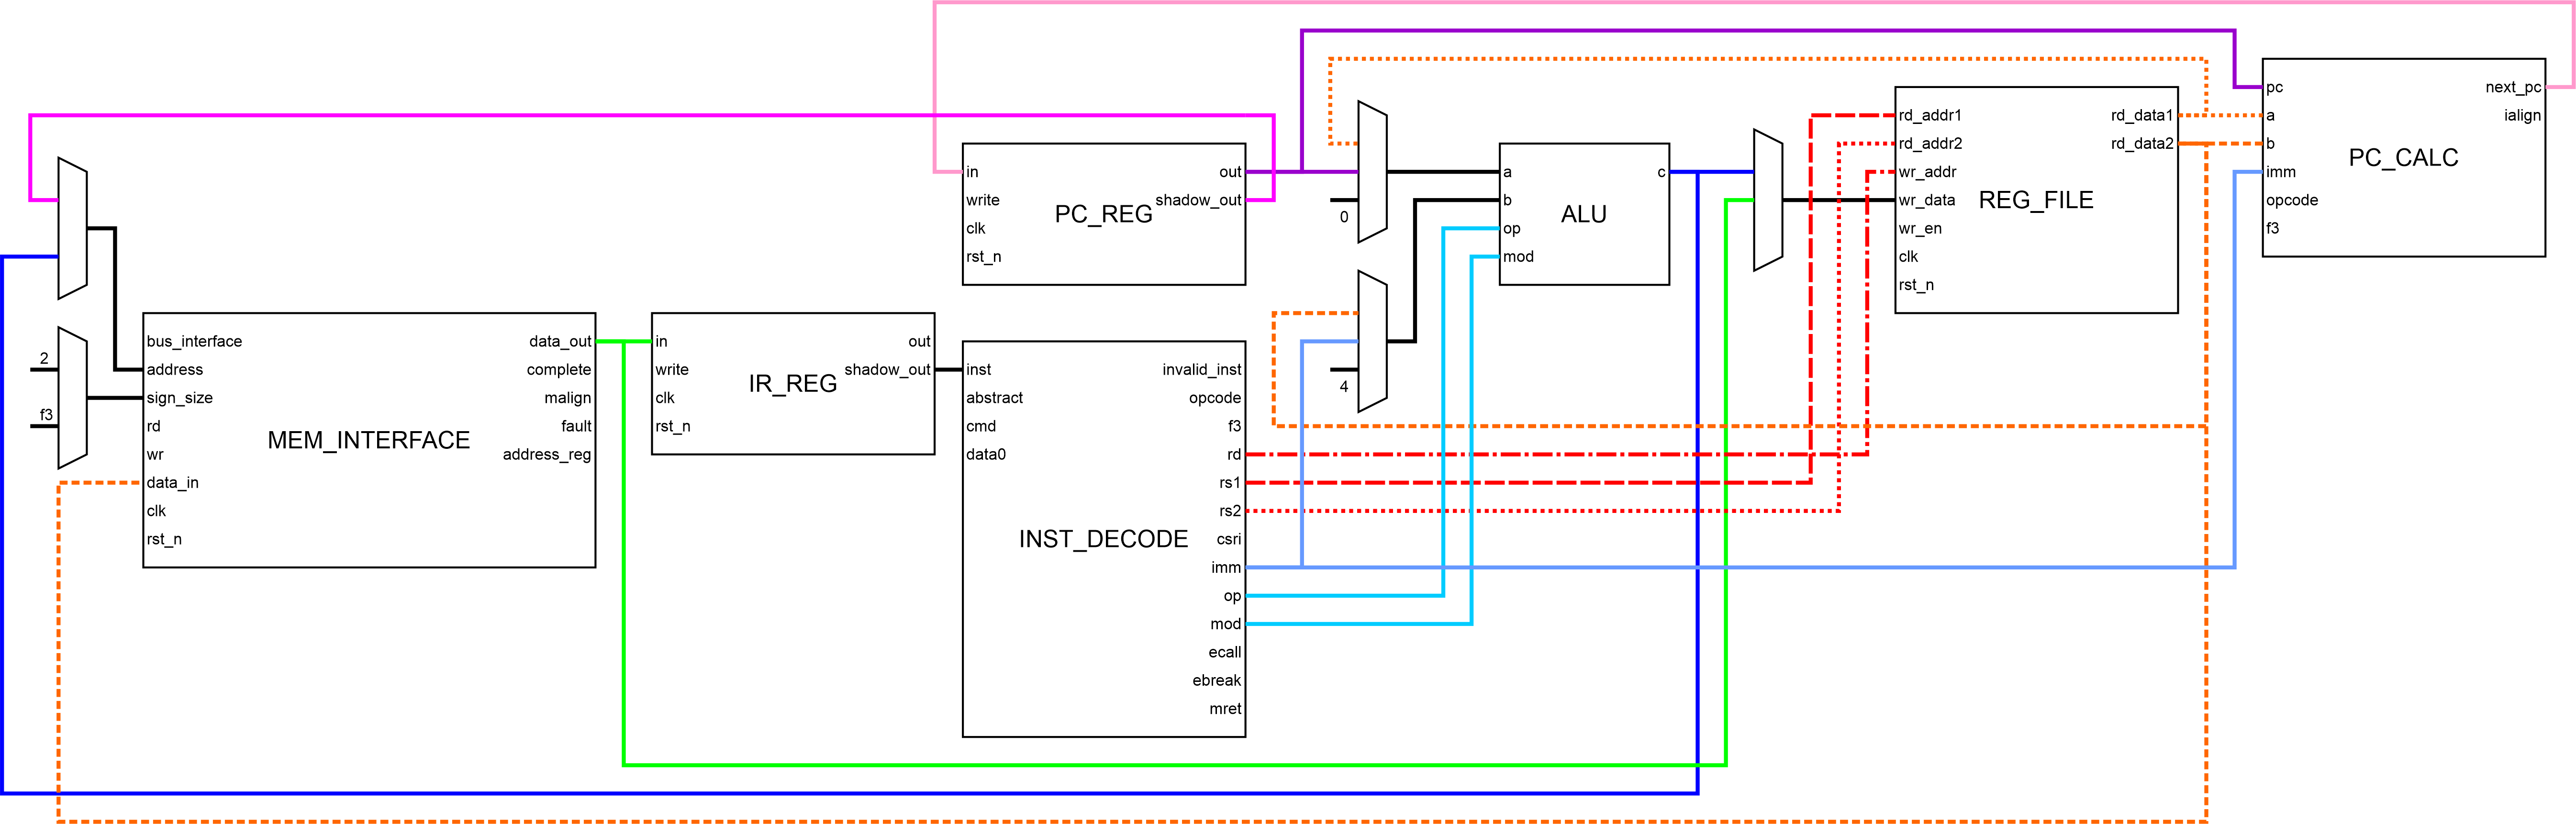
\includegraphics[width=0.945\textheight,angle=90]{data}
	\caption{Дијаграм путање података}
	\label{fig:data}
\end{figure}

\section{Управљачка јединица}

Неопходно је да управљачка јединица буде реализована Милијевим аутоматом стања јер управљачки сигнали зависе од операционог кода инструкције који се сазнаје у истом такту када и управљачки сигнали треба да буду подешени. Управљачка јединица је реализована директно у језику за опис хардвера, ово програмеру даје комфор сличан писању микропрограмске управљачке јединице док је резултујући хардвер након процеса синтезе сличнији ожиченој реализацији.

\lstinputlisting[language=Verilog, caption=Контролни сигнали управљачке јединице,label={lst:ctrls}]{listing/control_signals_if.svh}

Na почетку се могу видети дефиниције конкретних вредности управљачких сигнала за мултиплексере (два мултиплексера која одређују меморијску адресу и величину приступа имају заједнички управљачки сигнал). Након тога долазе дефиниције стања аутомата, за стање се користи 5 бита што је једнако ширини операционог кода инструкције и омогућава пресликавање вредности операционог кода у одговарајуће стање аутомата. Поред стања за сваки имплементирани операциони код, аутомат поседује још 6 стања: по два за инструкције читања и писања меморије, стање које припрема језгро за извршење прве инструкције и псеудостање које означава први такт извршавања инструкције.

Стања \textbf{LOAD\_1} и \textbf{STORE\_1} означавају други такт извршавања инструкције читања и писања меморије респективно. Стања \textbf{LOAD\_W} и \textbf{STORE\_W} су идентична стањима \textbf{LOAD} и \textbf{STORЕ} осим што не врше понован упис у \textbf{IR\_REG}. Аутомат улази у ова стања уколико му је линијом \textbf{inhibit} забрањено извршавање операција на магистрали, и у њима остаје док успешно не изврши тражену операцију, након чега прелази у \textbf{LOAD\_1} и \textbf{STORE\_1} респективно.
Стање \textbf{PROLOGUE} доводи језгро у стање у којем може следећег такта да почне са извршавањем инструкције. Ово стање врши дохватање инструкције из меморије са адресе која се тренутно налази у \textbf{PC\_REG}-у, и тиме гарантује испуњеност предуслова за извршавање инструкције (корак \ref{itemone} извршавања првог такта инструкције) уколико приступ меморији успе. Стање \textbf{PROLOGUE} се такође користи слично стањима \textbf{LOAD\_W} и \textbf{STORE\_W} уколико дохватање инструкције не успе. \textbf{DISPATCH} представља псеудостање је се систем никада неће наћи у том стању, већ вредност у регистру стања означава да се контролни сигнали понашају као да је систем у стању које је једнако операционом коду инструкције.

На крају примера кода \ref{lst:ctrls} се налази дефиниција интерфејса који садржи улазне и излазне контролне сигнале. Улазни сигнали су операциони код инструкције, као и информација да ли је приступ меморији успео (ово се односи само на линију \textbf{inhibit}, остале грешке се детектују на други начин). Излазни сигнали управљају уписом у \textbf{PC\_REG}, \textbf{IR\_REG} и \textbf{REG\_FILE}, читањем и уписом у меморију, као и избором сигнала на четири мултиплексера који су део путање података. У прилогу \ref{sec.control} се налази упрошћени код управљачке јединице.

\section{\textit{Zicsr} екстензија}

Екстензија \textit{Zicsr} прописује адресни простор од 4096 контролних и статусних регистара којима се приступа посебним инструкцијама које атомично читају и модификују те регистре регистарским директним или непосредним адресирањем. Ова функционалност је имплементирана у компоненти \textbf{CSR} која има следеће портове од интереса:
\begin{itemize}
	\item \textbf{csr\_interface}, интерфејс који остатак језгра користи да чита и уписује у контролне и статусне регистре.
	\item \textbf{rs}, adresa регистра опште намене чија вредност се уписује.
	\item \textbf{reg\_in}, вредност регистра опште намене чија вредност се уписује.
	\item \textbf{imm\_in}, вредност непосредног операнда који се уписује.
	\item \textbf{addr}, адреса контролног и статусног регистра који се уписује.
	\item \textbf{f3}, операција која се врши над регистром (уписивање, постављање бита или уклањање бита) и адресирање (регистарско директно или непосредно).
	\item \textbf{write}, контролни сигнал који врши упис у контролни и статусни регистар.
	\item \textbf{csr\_out}, излазни сигнал који представља вредност изабраног контролног и статусног регистра.
	\item \textbf{invalid}, излазни сигнал који означава да је дошло до грешке (непостојећи регистар или упис у заштићен регистар).
	\item \textbf{conflict}, излазни сигнал који означава да је у току упис у регистар који би такође био промењен при прихватању захтева за прекид.
\end{itemize}

Како постоји велики број ових регистара у великој мери су коришћени макрои да генеришу исти хардвер за сличне регистре, ови макрои се налазе у фајлу \textbf{csr.svh} чија је скраћена верзија испод.
\lstinputlisting[language=Verilog, caption=Пример макроа коришђених у \textbf{CSR} компоненти,label={lst:csr}]{listing/csr.svh}

Сама компонента \textbf{CSR} проверава да ли постоји регистар на датој адреси користећи један сигнал типа ожичено или, потом проверава да ли је покушан упис у регистар намењен само за читање (највиша два бита адресе су $11$) и уколико је потребно пријављује грешку. Остатак компоненте имплементира саме регистре коришћењем макроа приказаних на примеру кода \ref{lst:csr}, као и бројаче циклуса и извршених инструкција и системски тајмер. Системски тајмер се састоји од два меморијски мапирана регистра ширине 64 бита, они су имплементирани коришћењем \textbf{periph\_mem\_interface} компоненте која је раније описана. Бројачи циклуса и инструкција су имплементирани користећи исти интерфејс који остатак језгра користи да интерагује са контролним и статусним регистрима. Тај интерфејс се састоји од три линије за сваки регистар које се могу видети у макроу \textbf{CSRGEN\_\_GENERATE\_INTERFACE}. Линија са суфиксом \textbf{\_reg} представља вредност регистра, линија са суфиксом \textbf{\_in} представља вредност коју језгро жели да упише у тај регистар и линија са суфиксом \textbf{\_write} је активна у такту у коме језгро жели да упише нову вредност у тај регистар.

\lstinputlisting[firstline = 1, lastline = 21,language=Verilog, caption=Пример имплементације контролних и статусних регистара коришћењем макроа]{listing/csr.sv}

\section{Обрада прекида}

Имплементирано језгро подржава прекиде и изузетке\footnote{\рисцв{} спецификација прекидима класификује екстерне асинхроне догађаје, док су изузеци синхрони догађаји који су најчешће последица грешке при извршавању инструкције.} и врши њихову обраду у складу са привилегованом спецификацијом \cite{priv_spec}.

Већина логике за обраду прекида се налази у компоненти \textbf{INT\_CTL} док је поред тога потребна само минимална модификација путање података и управљачке јединице.
Модификација путање података је приказана на слици \ref{fig:mod}. Модификација управљачке јединице се састоји од извршавања следећих акција уколико је дошло до изузетка:
искључивање контролних сигнала који мењају стање (\textbf{write\_rd}, \textbf{write\_csr} и \textbf{mem\_write}), активација сигнала за упис \textbf{PC\_REG}-а када је дошло до изузетка (сигнал \textbf{write\_pc\_ex}), учитавање следеће инструкције макроом \textbf{CONTROL\_\_READ\_INST} и прелазак у стање \textbf{DISPATCH} или \textbf{PROLOGUE} у зависности да ли је дохватање инструкције успело. Уколико се прихвата прекид тренутна инструкција се правилно завршила те нема потребе за претходним операцијама.

\begin{wrapfigure}{l}{0.5\textwidth}
	\centering
	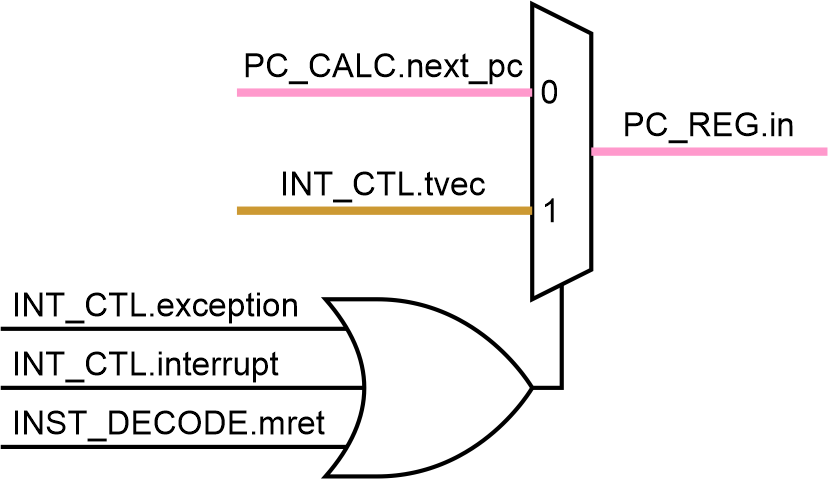
\includegraphics[width=0.5\textwidth]{mod}
	\caption{Модификација путање података}
	\label{fig:mod}
\end{wrapfigure}

\textbf{INT\_CTL} компонента врши детекцију изузетака и прекида, одређује адресу прекидне рутине и ажурира командне и статусне регистре од интереса.
Детекција изузетака је прилично једноставна, потребно је упарити линију која обавештава да је изузетак настао са тренутним стањем процесора како би се ближе одредило о ком изузетку је реч, нпр. приступ непостојећој меморији резултује једним од три изузетка дефинисаних у спецификацији \cite{priv_spec}: \textit{Instruction access fault}, \textit{Load access fault} или \textit{Store/AMO access fault}. Детекција прекида је такође једноставна, треба проверити линију која обавештава о захтеву за прекид и одговарајуће бите контролних и статусних регистара који маскирају појединачне или све прекиде. Сама одлука о скакању на прекидну рутину је нешто комплекснија и разматрају се још три услова. Да би се при обради прекида скочило на прекидну рутину потребно је да:
\begin{enumerate}
	\item Постоји захтев за прекид који није маскиран или постоји захтев за немаскирајући прекид.
	\item Уколико је у питању обичан прекид, прекиди нису глобално маскирани или уколико је у питању немаскирајући прекид, процесор тренутно не извршава прекидну рутину немаскирајућег прекида.
	\item Процесор тренутно извршава последњи такт инструкције.
	\item Тренутна инструкција не врши упис у неки од регистара чије вредности се ажурирају при скоку на прекидну рутину.
\end{enumerate}

Провера да ли процесор тренутно обрађује прекидну рутину немаскирајуђег прекида постоји зато што су све линије осетљиве на ниво што доводи до поновног скока на исту прекидну рутину након извршене једне инструкције прекидне рутине. Код обичних прекида ово је решено постављањем бита који глобално омогућава прекиде на 0 при скоку на прекидну рутину. Како сличан бит за немаскирајуће прекиде не постоји у спецификацији\footnote{Што је и логично, спецификација дефинише архитектуру тј. делове процесора доступне кориснику, што овај бит не би требао да буде. Такође спецификација намерно даје одређену слободу имплементацијама по питању обраде немаскирајућих прекида.}, у овој имплементацији је тај бит додат. Како је у питању само један бит чија се вредност враћа на 0 при извршавању прве инструкције повратка из прекидне рутине, потенцијално може настати проблем уколико се нека друга прекидна рутина угнезди унутар рутине немаскирајућег прекида, како је овај сценарио изузетно мало вероватан, није имплементирано боље решење, већ је неопходно да програмер буде свестан ове ситуације.

Прекиди се прихватају само на крају инструкције јер то значајно олакшава имплементацију а у општем случају одлаже прихватање прекида максимално један такт.
Разматрана је опција за прихватање прекида док је језгро у стању \textbf{PROLOGUE} као резултат активне линије \textbf{inhibit} међутим то би поприлично компликовало имплементацију а умањило би кашњење прихватања прекида за само један до два сигнала такта, иако језгро може провести произвољно велики број тактова у стању \textbf{PROLOGUE}. То је зато што ће језгро свакако провести исти број тактова у стању \textbf{PROLOGUE} и уколико одмах прихвати прекид јер и дохватање прве инструкције прекидне рутине захтева успешан приступ меморији. Тако да је једина разлика у кашњењу да ли ће се након уклањања активне вредности линије \textbf{inhibit} извршити једна додатна инструкција или не. Један изузетак овог правила је тај да се прекид може прихватити уколико се десио изузетак након првог такта инструкције која приступа меморији, то је зато што по спецификацији прекиди имају већи приоритет од изузетака а како инструкција која генерише изузетак не мења стање процесора безбедно је прихватити прекид уколико је адреса повратка из прекидне рутине инструкција која је изазвала прекид. Ово важи и за изузетке генерисане у последњем такту инструкције, међутим тада је правило о последњем такту инструкције испоштовано и једина разлика је адреса повратка из прекидне рутине.

Последњи случај у коме неће доћи до скока на прекидну рутину је уколико се тренутно извршава инструкција која врши упис у неки од контролних и статусних регистара који се ажурирају при скоку на прекидну рутину. Ово се примарно односи на регистар \textbf{\acrshort{MSTATUS}} је проширено и на остале регистре (\textbf{\acrshort{MCAUSE}}, \textbf{\acrshort{MTVAL}} и \textbf{\acrshort{MEPC}}). Овај сигнал генерише компонента \textbf{CSR} и постоји због једног ивичног случаја\footnote{Можда постоје и други ивични случајеви али један је довољан да објасни зашто је овај услов неопходан.} у коме програм уписује 0 у бит који омогућава све прекиде (бит \textbf{\acrshort{MIE}} регистра \textbf{\acrshort{MSTATUS}}), како ће упис бити видљив језгру тек следећег такта, прекид се прихвата (ово само по себи није проблем, рећићемо да је прекид прихваћен пре комплетног извршења те инструкције) међутим у поље \textbf{\acrshort{MPIE}} регистра \textbf{\acrshort{MSTATUS}} се уписује тренутна вредност бита \textbf{\acrshort{MIE}} а не 0 која се тренутно уписује. Што значи да ће, када се при повратку из прекидне рутине у бит \textbf{\acrshort{MIE}} упише вредност бита \textbf{\acrshort{MPIE}}, она бити као да се инструкција након које је прихваћен прекид није десила, што може резултовати у томе да су прекиди омогућени иако не би требали да буду. Иако за овај ивични случај сигурно постоје и алтернативна решења ово решење је поприлично једноставно и у најгорем случају одлаже прекид један такт.

Следећи корак при обради прекида и изузетака је одређивање уколико постоји више разлога за скок који ђе бити испоштован. Већ је споменуто шта се дешава уколико се истовремено десе изузетак и прекид, међутим још један разлог за скок који обрађује ова компонента је повратак из прекидне рутине инструкцијом \textbf{MRET}. Табела \ref{tab:int} приказује исход сваке комбинације. Изузеци и прекиди се међусобно приоритирају по фиксним приоритетима дефинисаним у спецификацији \cite{priv_spec}.

\begin{table}[h!]
	\centering
	\caption{Исход комбинација прекида, изузетака и повратка из прекидне рутине}
	\label{tab:int}
\begin{tabular}{|c|c|c|c|c|}
	\hline
	Изузетак & Прекид & Повратак из прекидне рутине & Акција & \textbf{\acrshort{MEPC}} = \\
	\hline
	* &  &  & Изузетак & \textbf{pc} \\
	\hline
	& * &  & Прекид & \textbf{next\_pc} \\
	\hline
	&  & * & Повратак & / \\
	\hline
	* & * &  & Прекид & \textbf{pc} \\
	\hline
	* &  & * & Изузетак & \textbf{pc} \\
	\hline
	& * & * & Повратак & / \\
	\hline
	* & * & * & Прекид & \textbf{pc} \\
	\hline
\end{tabular}
\end{table}\newpage

Одређивање адресе на коју се скаче је једноставно, уколико је у питању повратак из прекидне рутине, скаче се на адресу у \textbf{\acrshort{MEPC}} регистру, уколико је у питању изузетак или прекид и прекиди нису векторисани скаче се на адресу у регистру \textbf{MTVEC} поравнату на 4 бајта, уколико су прекиди векторисани на адресу се додаје код узрока прекида померен за 2 бита улево.

\textbf{INT\_CTL} такође ажурира следеђе контролне и статусне регистре:
Регистар \textbf{\acrshort{MIP}} се ажурира сваког такта са вредностима линија захтева за прекид.
При уласку у прекидну рутину бит \textbf{\acrshort{MPIE}} се ажурира тренутном вредношћу бита \textbf{\acrshort{MIE}} а \textbf{\acrshort{MIE}} се поставља на 0.
При повратку из прекидне рутине овај процес је обрнут, \textbf{\acrshort{MIE}} добија вредност \textbf{\acrshort{MPIE}} а \textbf{\acrshort{MPIE}} се поставља на 1.
Регистар \textbf{\acrshort{MEPC}} се ажурира при уласку у прекидну рутину по табели \ref{tab:int}.
Регистри \textbf{\acrshort{MCAUSE}} и \textbf{\acrshort{MTVAL}} se ажурирају при уласку у прекидну рутину са кодом узрока прекида и описом изузетка (уколико је применљиво) респективно.
Уколико се користи \textbf{\acrshort{MTVAL}} најчешће има вредност меморијске адресе која је изазвала изузетак или вредности инструкције која је невалидна.